% ----- formatovani dokumentu -----------------------------------------------
\documentclass[12pt,a4paper,titlepage,final]{report}
\usepackage[utf8]{inputenc}
\usepackage[T1, IL2]{fontenc}
\usepackage{graphicx}
\usepackage{epstopdf}
\usepackage[margin=2cm]{caption}
\usepackage[top=3cm, left=2cm, right=2cm, text={17cm, 24cm}, ignorefoot]{geometry}
\usepackage{color}
\usepackage{url}
\usepackage{setspace}
\singlespacing
\usepackage[square, numbers]{natbib} 
\pagestyle{plain}
\pagenumbering{arabic}
\setcounter{page}{1}
\setcounter{secnumdepth}{-1}
\setlength{\parindent}{1cm}	
\usepackage{natbib}
\usepackage{float}
\usepackage[hyphenbreaks]{breakurl}

\providecommand{\uv}[1]{\quotedblbase #1\textquotedblleft}

% ----- vyberte jazyk -------------------------------------------------------
\usepackage[english,czech]{babel}
%\usepackage[english]{babel}

% ----- dopiste titulky -----------------------------------------------------
\newcommand\Course{Počítačová grafika}
\newcommand\WorkTitle{Šachy pomocí ray-tracing}
\newcommand\AuthorA{Adam Jež}
\newcommand\AuthorAEmail{xjezad00@stud.fit.vutbr.cz}
\newcommand\AuthorB{Tomáš Mlynarič}
\newcommand\AuthorBEmail{xmlyna06@stud.fit.vutbr.cz}
\newcommand\AuthorC{Ivan Ševčík}
\newcommand\AuthorCEmail{xsevci50@stud.fit.vutbr.cz}
\newcommand\Faculty{Fakulta Informačních Technologií}
\newcommand\School{Vysoké Učení Technické v Brně}

\PassOptionsToPackage{hyphens}{url}
\usepackage[
pdftitle={\WorkTitle},
pdfauthor={\AuthorA, \AuthorB, \AuthorC},
bookmarks=true,
colorlinks=true,
breaklinks=true,
urlcolor=blue,
citecolor=blue,
linkcolor=blue,
unicode=true,
]
{hyperref}


% ----- titulni strana ------------------------------------------------------

\begin{document}
	\begin{titlepage}
	\begin{center}
		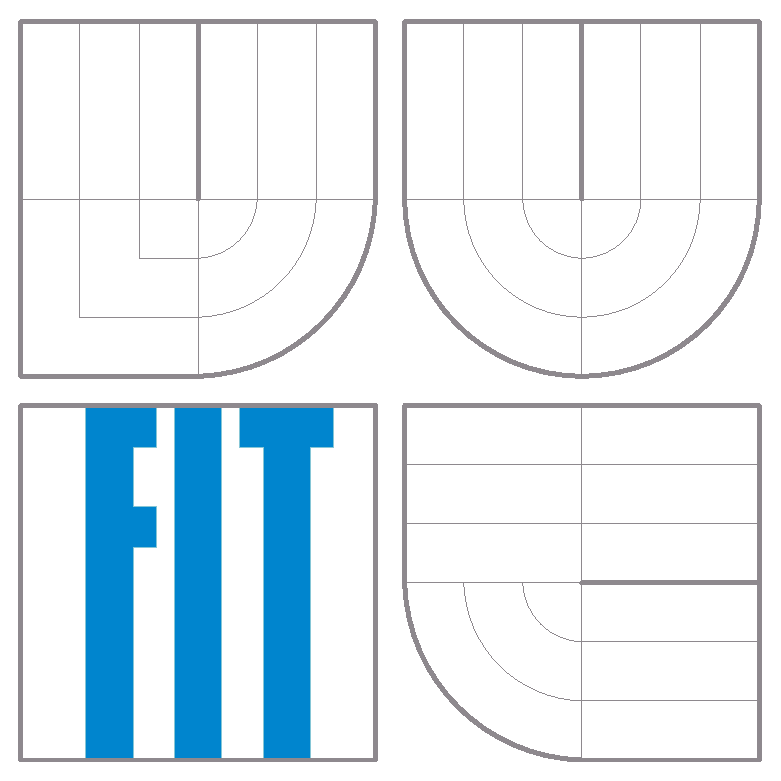
\includegraphics[height=5cm]{images/logo.eps}
	\end{center}
	\vfill
	\begin{center}
		\begin{Large}
			\Course\\
		\end{Large}
		\bigskip
		\begin{Huge}
			\WorkTitle\\
		\end{Huge}
	\end{center}
	\vfill
	\begin{center}
		\begin{large}
			\today
		\end{large}
	\end{center}
	\vfill
	\begin{flushleft}
		\begin{large}
			\begin{tabular}{lll}
				Autoři: & \AuthorA, & \url{\AuthorAEmail} \\
				        & \AuthorB, & \url{\AuthorBEmail} \\
				        & \AuthorC, & \url{\AuthorCEmail} \\
				& & \\
				& \Faculty \\
				& \School \\
			\end{tabular}
		\end{large}
	\end{flushleft}
\end{titlepage}		
	
% ----- obsah --------------------------------------------------------------
	
\tableofcontents

% ----- zadani -------------------------------------------------------------
\newpage
\chapter{Zadání}

Úlohou bylo implementovat metodu ray-tracingu\footnote{Ray-tracing - metoda  sledování paprsků} a s její pomocí vizualizovat scénu složenou ze šachovnice a šachových figurek. Důraz měl být kladen na kvalitu výsledného zobrazení a jevy, které se obtížně vizualizují pomocí klasických vykreslovacích technik. Dalším požadavkem bylo implementovat uložení stavu šachovnice, která by byla vhodná pro interakci se šachovým strojem nebo uživatelem přes GUI. Důležitá byla také parametrizovatelnost procesu vykreslování.

Vzhledem k účelu bylo žádoucí, aby překreslování bylo plynulé, proto byl také kladen důraz na optimalizace a další techniky urychlení výpočtu. Dále, pro prezentaci výsledků, bylo vhodné mít možnost zachytit snímek a uložit ho do souboru bez nutnosti dělat snímek celé obrazovky a poté ořezávat. 

Celkově bylo tedy nutné věnovat se v rámci projektu těmto částem:
\begin{itemize}
	\item Raytracer
	\begin{itemize}
	    \item Tvorba 3D primitiv a jejich skládání
		\item Odlesky a stíny
		\item Antialiasing
		\item Parametrizovatelnost
		\begin{itemize}
			\item Změna pohledu kamery
			\item Změna pozice světla
			\item Stupeň antialiasingu
			\item Úroveň odlesků
		\end{itemize}
	\end{itemize}
	\item Šachová partie
	\begin{itemize}
	    \item Tvorba modelů figurek a scény
		\item Vhodná reprezentace
		\item Možnost uložení do souboru
		\item Možnost uložit snímek 
	\end{itemize}
	\item Plynulost překreslování
	\begin{itemize}
		\item Profilování a optimalizace kritických částí
		\item Paralelizace výpočtu
	\end{itemize}
\end{itemize}

\chapter{Použité technologie}
Program byl napsán v jazyku \texttt{C\#} pro \texttt{.Net 4.5} a kromě knihovny \texttt{OpenTK} nevyžaduje ke svému běhu žádné další. Uživatelské rozhraní bylo implementováno pomocí frameworku \texttt{WinForms}. Ten je již poměrně zastaralý, ale díky přenositelnosti na jiné platformy, pro účely aplikace postačující.

Při vývoji bylo použito \texttt{Visual Studio 2015} a verzovací systém \texttt{git} s repozitářem na službě \texttt{GitHub}. Vývoj probíhal pod operačními systémy \texttt{Windows} a testování výsledného programu proběhlo také na systému \texttt{Linux}, kde bylo pro zkompilování použito \texttt{MonoDevelop}.


\begingroup
\let\clearpage\relax
\chapter{Použité zdroje}
Teorie ray-tracingu byla získána z přednášek předmětu PGR a ze stránky \cite{scratchapixel}. Projekt byl značně inspirován ray-tracerem Aurelius probíraném na přednáškách předmětu PGR \cite{aurelius}, který byl dále rozšiřován implementováním dalších 3D primitiv (konečný válec, kužel) a také pokročilejšími operacemi s těmito primitivy. Obecný kužel byl implementován pomocí rovnic uvedených v~přednášce ze zahraniční univerzity \cite{cone}. Dále rovnice pro odlesk byla přebrána ze stránek \cite{reflect} a~Phongův osvětlovací model byl ozřejmen pomocí webu \cite{phong}. Efektivní test průniku paprsku s~obalovacím kvádrem byl nalezen na stránce \cite{aabb}.

\endgroup

%---------------------------------------------------------------------------
\chapter{Nejdůležitější dosažené výsledky}
Aplikace byla implementována a optimalizována tak, aby dosažené výsledky byly co nejlepší z~hlediska krásy, aby bylo možno se scénou rozumně manipulovat a přitom překreslovací frekvence byla co nejvyšší.

\section{Krása výsledku}

Výsledného hezkého vizuálního efektu (viz obrázky \ref{fig:chess1}, \ref{fig:chess2}, \ref{fig:chess3}) bylo dosaženo pomocí Phongova osvětlovacího modelu, odlesků, odrazů, stínů a antialiasingu. Dále byly vytvořeny nevšední modely šachových figurek spojením 3D primitiv pomocí \texttt{Constructive Solid Geometry} (dále jen CSG) stromů. Přiřazení barvy, odlesků a dalších parametrů figurek a jiných objektů bylo voleno tak, aby celá scéna byla co nejzajímavější a byly prezentovány různé efekty povrchů.

\begin{center}
	\captionsetup{type=figure}
		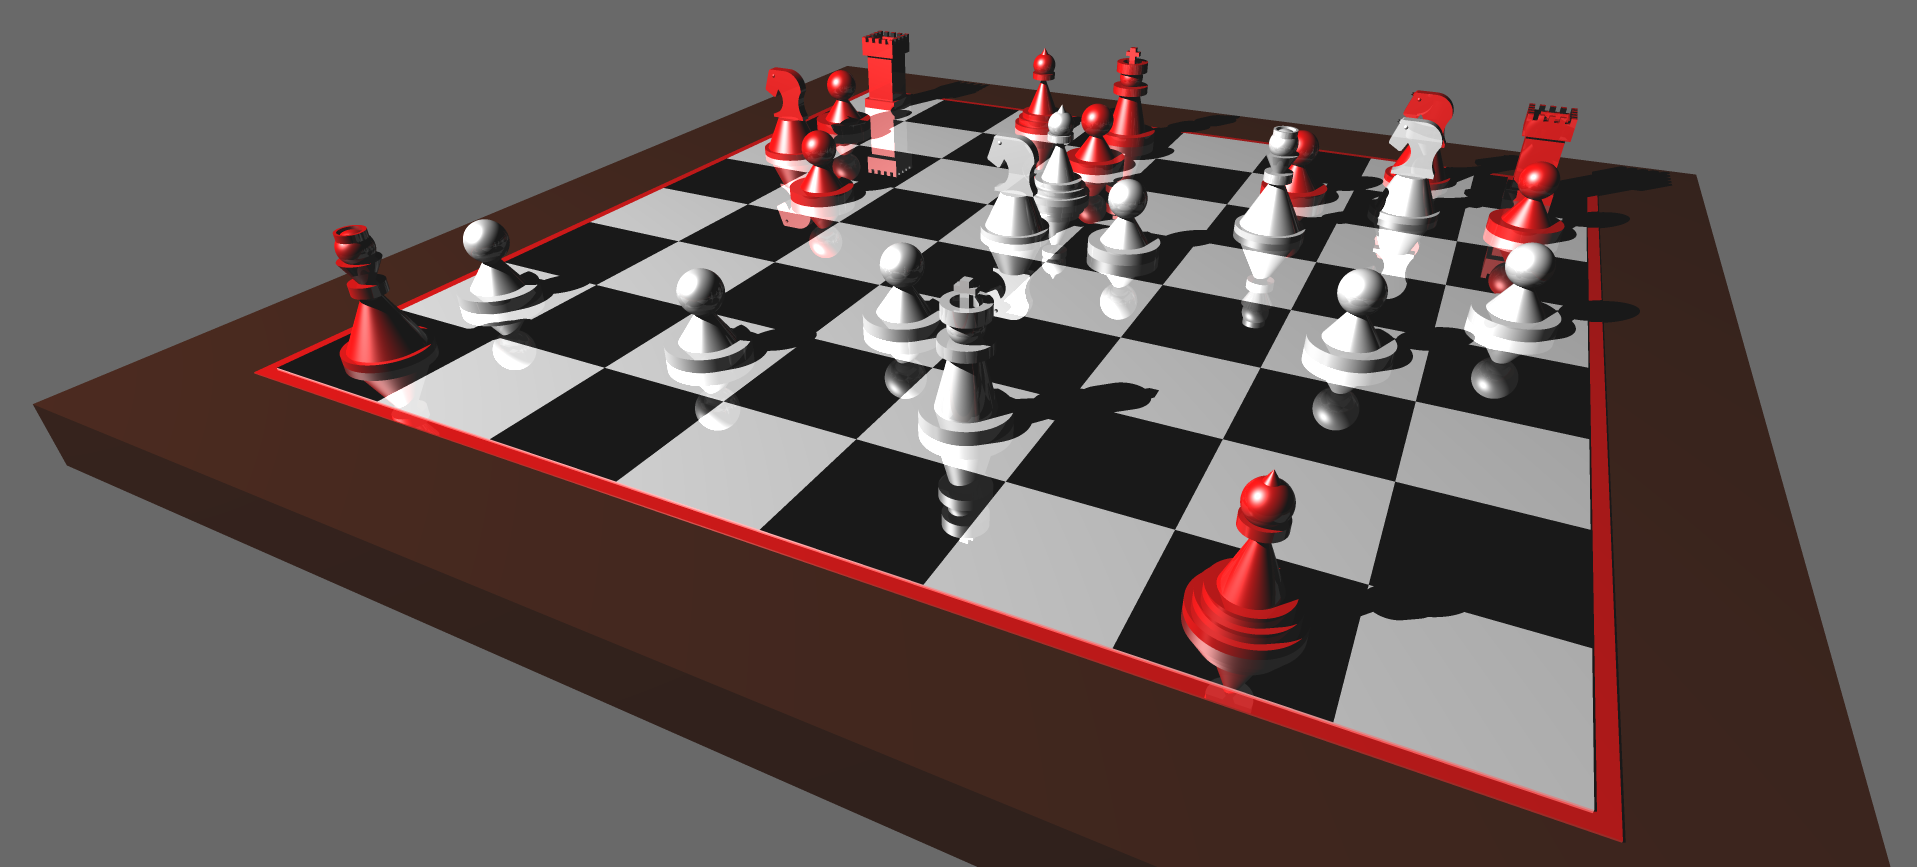
\includegraphics[width=0.8\linewidth]{images/scene1.png}
	\captionof{figure}{Základní vizualizace libovolné partie}
	\label{fig:chess1}
\end{center}

\begin{center}
	\captionsetup{type=figure}
	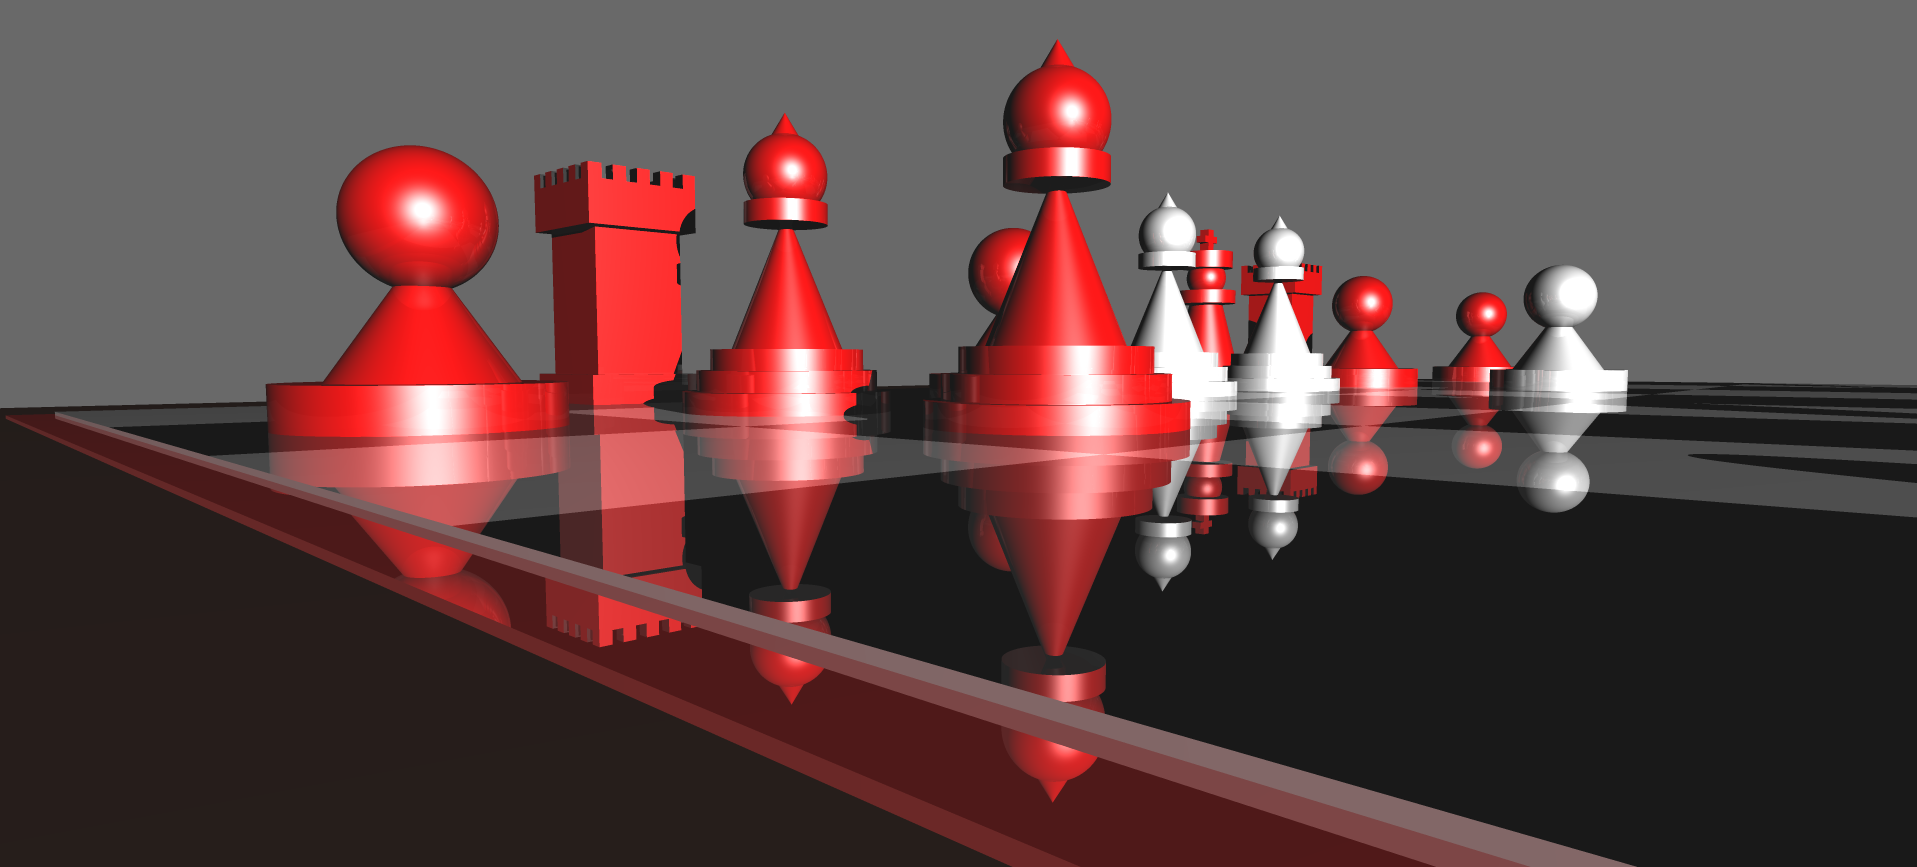
\includegraphics[width=0.8\linewidth]{images/scene2.png}
	\captionof{figure}{Různá míra odrazivosti materiálu}
	\label{fig:chess2}
\end{center}

\begin{center}
	\captionsetup{type=figure}
	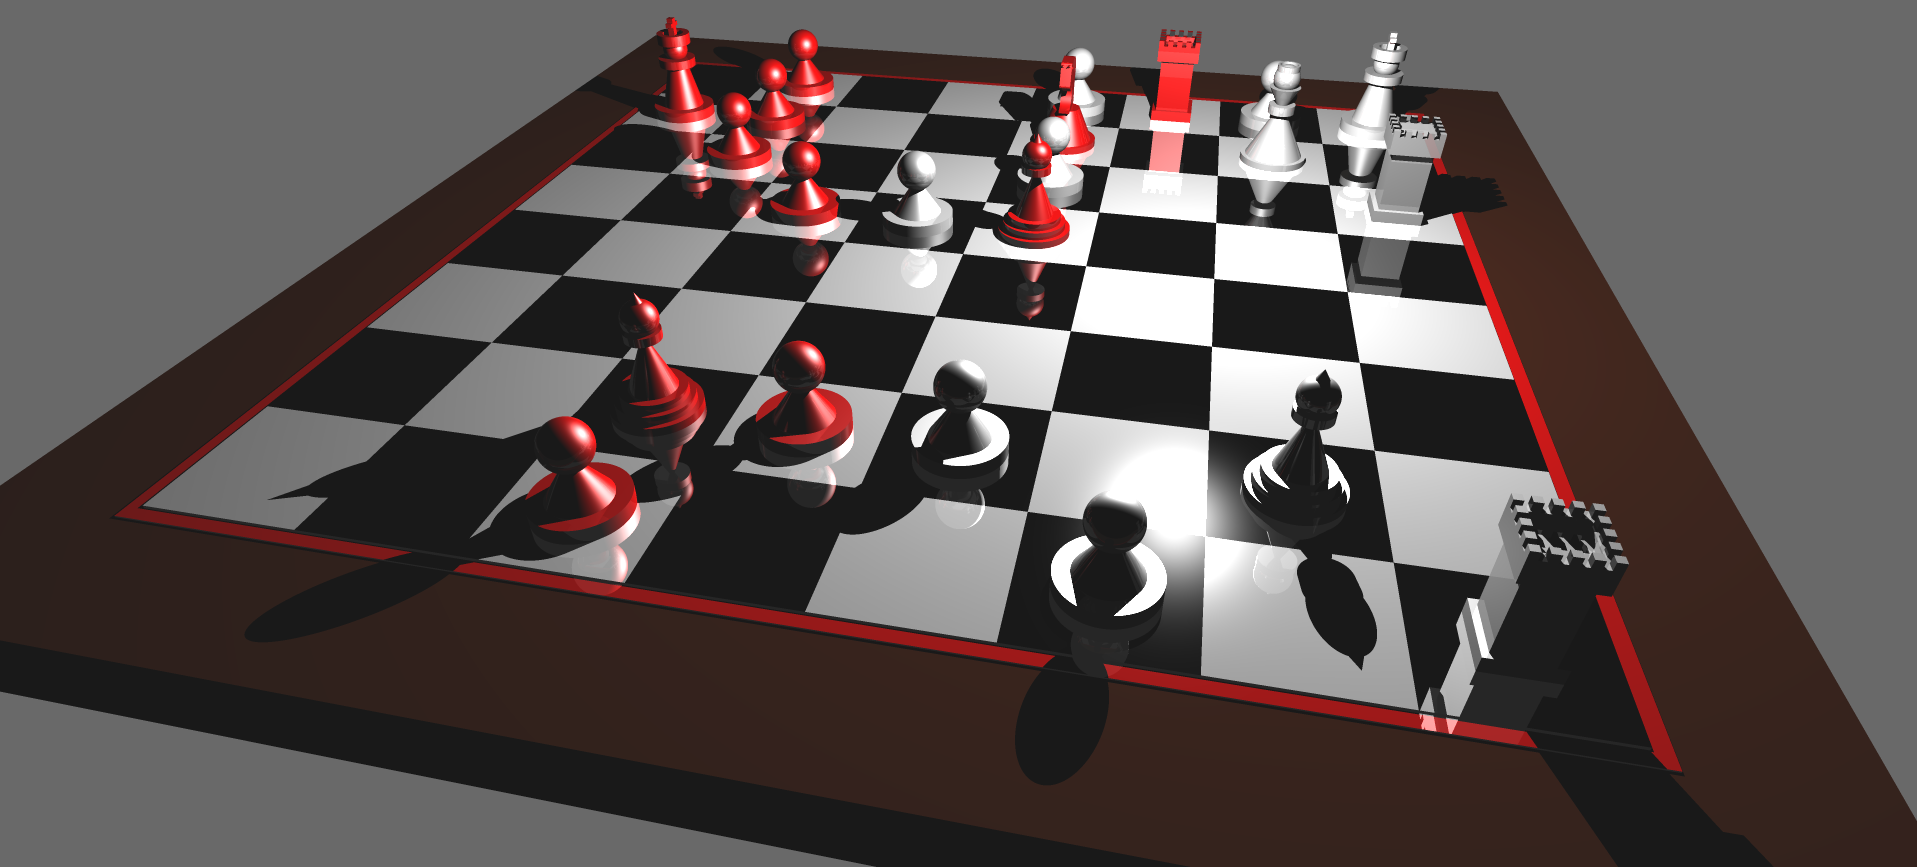
\includegraphics[width=0.8\linewidth]{images/scene3.png}
	\captionof{figure}{Různě vržené stíny}
	\label{fig:chess3}
\end{center}

\section{Intuitivní manipulace}
Se scénou je možné manipulovat přirozeným způsobem pomocí myši. Je možné kameru otáčet okolo bodu ve scéně, přibližovat nebo oddalovat kolečkem a také pohybovat se ve scéně podržením prostředního tlačítka.
Kombinace rotace a posunu podél osy kamery umožňuje přesun na libovolnou pozici ve 3D prostoru, i když pohyb myši po obrazovce poskytuje jen 2D souřadnice. 

Pomocí pravého tlačítka myši je také možné měnit pozici světla, a tedy interaktivně vizualizovat různé stíny a odlesky.

Jelikož metoda ray-tracing je velmi náročná a na některých přístrojích nemusí být možné pozorovat scénu v reálném čase, je také možno výše uvedené parametry měnit pomocí změny čísla v komponentách okna, a tudíž je možné přímo změnit souřadnice na požadované.

\section{Překreslovací frekvence}
\label{sec:fps}

Při prvním pokusu o vytvoření funkčního ray-traceru byl použit způsob popisu scény pomocí hraniční reprezentace, tj. síti trojúhelníků. Čas vytvoření jednoho snímku pro jednoduchý model konvice\footnote{Utah Teapot - viz \url{https://en.wikipedia.org/wiki/Utah_teapot}} bez jakýchkoliv efektů a pouze s plochým stínováním se pohyboval okolo 40 sekund. Na základě této zkušenosti byl proveden průzkum možností zobrazení modelů a zvolen byl způsob reprezentace pomocí CSG. Tento způsob urychlil samotný výpočet přibližně stonásobně. V principu se jedná o to, že bylo potřeba najít takové modely, které lze jednoduše popsat analytickými rovnicemi, pro které bylo možné spočítat průsečík a najít tak bod, na kterém světlo ve scéně dopadne. Pro další urychlení výpočtu byl zvolen způsob aproximace počítání průsečíků s modely ve scéně pomocí obalovacích těles, konkrétně \texttt{AABB}\footnote{AABB - Axis-aligned bounding box}. Nakonec byla také zavedena paralelizace výpočtu na CPU pomocí vláken, která ale neměla tak výrazný vliv na zrychlení.

Pro plynulou interakci s uživatelem však byl zaveden \emph{odlehčený} vykreslovací mód, jak je možné vidět na obrázku \ref{camera}, který se zapne při pohybu kamerou a vypne po dokončení změny. Po zapnutí se pak vykreslují pouze stínovaná obalovací tělesa, která pro uživatele obvykle stačí pro představu, kde ve scéně se kamera nachází a vykreslování je pak mnohem rychlejší. 

Dalším zrychlovacím mechanismem je použití cache objektů, např. v případě, že se neměnila pozice kamery. V tomto případě je možné znovu využít stejných paprsků jak při posledním vykreslování. Také je možné uložit pro další použití některé mezivýsledky z různých výpočtů.

\begin{figure}[H]
	\centering
	\captionsetup{type=figure}
	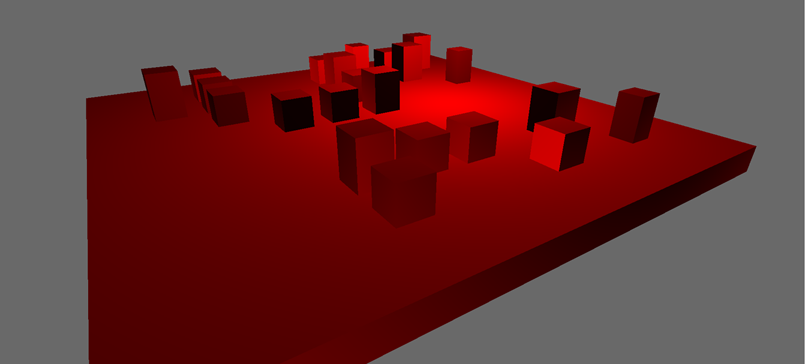
\includegraphics[width=0.8\linewidth]{images/camera.png}
	\captionof{figure}{Vykreslování během pohybu kamerou}
	\label{camera}
\end{figure}

Výsledkem těchto optimalizací je vcelku uspokojivá překreslovací frekvence vzhledem k~nárokům na prostředky počítače této metody vykreslování. Následující tabulka představuje rychlost překreslování programu na základě různých parametrů a rozlišení\footnote{Testování proběhlo na počítači s procesorem Intel i7-3630QM a 8 GB RAM}.

\begin{table}[H]
	\begin{center}
		\begin{tabular}{| l | c | c | c | c| c | c |}
			\hline
			Rozlišení & $600\times400$ & $600\times400$ & $600\times400$ & $600\times400$ & $600\times400$ & $1917\times867$
			\\ \hline
			
			Počet vláken & 1 & 8 & 8 & 8 & 8 & 8
			\\ \hline
			
			Stupeň odrazivosti & 0 & 0 & 2 & 2 & 2 & 2
			\\ \hline
			
			Antialiasing & vypnutý & vypnutý & vypnutý & vypnutý & $2\times2$ & vypnutý
			\\ \hline
			
			Kamera v pohybu & Ne & Ne & Ne & Ano & Ne & Ne
			\\ \hline
			
			\textbf{FPS} & 0.81 & 2,6 & 1,42 & 5,8 & 0,34 & 0,23
			\\ \hline
		\end{tabular}
	\end{center}	
	\caption{Překreslovací frekvence pro různé konfigurace}  
\end{table}

%---------------------------------------------------------------------------
\chapter{Práce na projektu}

\section{Rozdělení práce v týmu}

\begin{itemize}
\item \textbf{\AuthorA}: serializace scény a šachové partie, vytvoření modelů figurek + scény 
\item \textbf{\AuthorB}: ray-tracer, GUI, dokumentace
\item \textbf{\AuthorC}: základ projektu, CSG, paralelizace,  dokumentace
\end{itemize}

%---------------------------------------------------------------------------
\section{Co bylo nejpracnější}

\begin{itemize}
\item \textbf{\AuthorA}: vytvoření hezky vyhlížejících modelů pro figurky a scénu
\item \textbf{\AuthorB}: nedoplést se při skládání metody ray-traceru, tzn. který vektor se sčítá a násobí jiným
\item \textbf{\AuthorC}: spočítat rovnice průsečíků 3D primitiv a skládání primitiv do CSG stromů
\end{itemize}


%---------------------------------------------------------------------------
\section{Zkušenosti získané řešením projektu}

Při řešení projektu jsme zjistili, že když se projekt dobře naplánuje a rozdělí (celkem podrobně) úkoly, pak řešení projektu jde plynulým tempem dopředu. Také jsme zjistili, že neznalost problematiky může vést k nadbytečnému předělávání kódu (viz strana \pageref{sec:fps}).

Z hlediska počítačové grafiky jsme si odzkoušeli jeden ze způsobů reprezentace modelů ve scéně, tj. CSG. Také jsme si uvědomili rozdíly ve vykreslovacích metodách a k čemu se hodí jednotlivé metody používat (tj. pomocí ray-tracingu nikdy nedostaneme realtime aplikaci, ale na druhou stranu dosáhneme téměř realisticky vyhlížejících modelů pomocí jednoduchého programu). 

Z oblasti matematiky jsme pak byli nuceni osvěžit si vektorovou algebru a připomenout si analytické popisy 3D primitiv a operace s nimi.

%---------------------------------------------------------------------------
\chapter{Autoevaluace}

\paragraph{Technický návrh (55 \%):} (analýza, dekompozice problému, volba
vhodných prostředků, $\ldots$) 

Slabě provedena analýza problematiky ray-tracingu, naopak vhodný výběr prostředků (\texttt{git}, \texttt{C\#}, \texttt{OpenTK}), které umožňovaly efektivní práci nad problémem místo zabýváním se primitivními problémy (např. řešením konfliktních změn mezi pracovníky, konstrukcí jazyka nižší úrovně apod.).

\paragraph{Programování (60 \%):} (kvalita a čitelnost kódu, spolehlivost běhu,
obecnost řešení, znovupoužitelnost, $\ldots$)

Čitelnost kódu není světlou stránkou projektu, nicméně díky způsobu ukládání a načítání informací o scéně je možné načíst jakoukoliv scénu šachů, volit jednotlivé prvky scény libovolně (pozici světla a kamery, barvy hráčů atd.), dále jednoduchou úpravou je ray-tracer schopen zobrazit libovolné modely, které jsou popsané pomocí CSG stromů. 


\paragraph{Vzhled vytvořeného řešení (75 \%):} (uvěřitelnost zobrazení,
estetická kvalita, vhled GUI, $\ldots$)

GUI bylo kvůli přenositelnosti na jiné systémy konstruováno velmi jednoduše, nicméně rozmístění komponent a reakce na uživatelovy podněty by měly být přehledné a srozumitelné. Výsledná vizualizace šachů je velmi hezká a scéna budí dojem realističnosti. 

\paragraph{Využití zdrojů (65 \%):} (využití existujícího kódu a dat, využití
literatury, $\ldots$)

Při tvorbě projektu jsme se inspirovali zdrojovým kódem programu Aurelius, dále spíše teoretickým popisem problematiky nebo pseudokódem.

\paragraph{Hospodaření s časem (90 \%):} (rovnoměrné dotažení částí projektu,
míra spěchu, chybějící části řešení, $\ldots$)

Projekt byl z hlediska času rozvržen vhodně, práce probíhala na začátku semestru, pak v průběhu půlsemestrálních zkoušek byla pauza a ke konci semestru a po načerpaní informací z přednášek byl projekt dokončen.

\paragraph{Spolupráce v týmu (80 \%):} (komunikace, dodržování dohod, vzájemné
spolehnutí, rovnoměrnost, $\ldots$)

Komunikace probíhala vesměs skrze internet s občasnými schůzkami, kde se obvykle probraly problémy z předchozí iterace a prodiskutovaly se úkoly, které bylo potřeba dále řešit. Každý z řešitelů vložil přibližně rovnoměrné úsilí do projektu, ať už programátorsky, organizačně či teoreticky.

\paragraph{Celkový dojem (75 \%):} (pracnost, získané dovednosti, užitečnost,
volba zadání, cokoliv, $\ldots$)


Volba zadání se jevila jako vhodná, protože se jednalo z našeho hlediska o neprobádanou oblast počítačové grafiky, přičemž projekt zůstával po celou dobu zajímavý.

%---------------------------------------------------------------------------
\chapter{Ovládání vytvořeného programu}
Aplikaci je možné přeložit a spustit pomocí programu Visual Studio. V případě zkopírování přeložených knihoven aplikace je možné ji spustit i na jiných počítačích bez překladového systému.

\subsection{Nahrávání scény}
Pro zobrazení scény, tj. vyrenderování stavu šachů, slouží tlačítko \uv{Render}, které ve výchozím stavu zobrazí základní rozmístění šachovnice. Toto rozmístění je možné upravovat na základě načtení souboru, který obsahuje informace o scéně.
Dále je možné načtenou scénu uložit nebo exportovat jako obrázek.

\subsection{Manipulace se scénou}
Manipulace je možná pomocí myši. Levým tlačítkem je možné rotovat okolo bodu ve scéně, prostředním posouvat se ve scéně,
pravé tlačítko pak slouží ke změně souřadnic pozice světla. Druhým způsobem, například při velkém rozlišení nebo zapnutém antialiasingu, je možné ovládat scénu pomocí zadávání souřadnic kamery a světla.

\subsection{Parametrizace}
Nastavení parametrů je možné pomocí klasických komponent grafických aplikací. Všechny tyto parametry reagují na změnu za běhu vykreslování, kromě nastavení počtu vláken výpočtu, u~kterého je nutné vykreslování zastavit a znovu spustit.

%---------------------------------------------------------------------------
\chapter{Doporučení pro budoucí zadávání projektů}

Zajímavé na projektu bylo jeho jednoduché zadání, dle kterého jsme si mohli projekt dospecifikovat sami. 


%---------------------------------------------------------------------------

\bibliographystyle{plain}
\bibliography{reference}
\addcontentsline{toc}{chapter}{Literatura}

\end{document}

